\documentclass[10pt]{article}
\usepackage[left=1.5cm, right=1.5cm, top=0.8in, bottom=0.7in]{geometry}
\usepackage{fancyhdr}
\pagestyle{fancy}
\usepackage[most,breakable]{tcolorbox}
\usepackage{pdfcol,xcolor}
\usepackage{tikz}
\usepackage[linesnumbered,ruled,vlined]{algorithm2e}
%\usepackage{url}
\usepackage{dsfont}
\usepackage{amssymb,amsmath}
\usepackage{xspace}
\usepackage[normalem]{ulem}
\usepackage{bm}
\usepackage[breaklinks=true,colorlinks,linkcolor=magenta,urlcolor=magenta,citecolor=black]{hyperref}
\usepackage{cleveref}
\usepackage{xpatch}
\xpretocmd{\algorithm}{\hsize=\linewidth}{}{}

\newtcolorbox[auto counter]{exercise}[1][]{%
	colback=yellow!10,colframe=red!75!black,coltitle=white,use color stack,enforce breakable,enhanced,fonttitle=\bfseries,before upper={\parindent15pt\noindent}, title={\color{white}Exercise~\thetcbcounter: #1}}
\pagecolor{yellow!10}

\lhead{
\textbf{University of Waterloo}
}
\rhead{\textbf{2024 Spring}
}
\chead{\textbf{
CS480/680
 }}
\lfoot{}
\cfoot{\textbf{Yao-Liang Yu (yaoliang.yu@uwaterloo.ca) \textcopyright 2024}}

\newcommand{\RR}{\mathds{R}}
\newcommand{\sign}{\mathop{\mathrm{sign}}}
\newcommand{\argmin}{\mathop{\mathrm{argmin}}}
\newcommand{\zero}{\mathbf{0}}
\newcommand{\one}{\mathbf{1}}
\newcommand{\bv}{\mathbf{b}}
\newcommand{\wv}{\mathbf{w}}
\newcommand{\xv}{\mathbf{x}}
\newcommand{\Xv}{\mathbf{X}}
\newcommand{\Yv}{\mathbf{Y}}
\newcommand{\zv}{\mathbf{z}}
\newcommand{\yv}{\mathbf{y}}
\newcommand{\rv}{\mathbf{r}}
\newcommand{\inner}[2]{\langle #1, #2 \rangle}
\newcommand{\red}[1]{{\color{red}#1}}
\newcommand{\blue}[1]{{\color{blue}#1}}
\newcommand{\magenta}[1]{{\color{magenta}#1}}
\newcommand{\green}[1]{{\color{green}#1}}
\newcommand{\xbs}{\bm{\mathsf{x}}}
\newcommand{\wbs}{\bm{\mathsf{w}}}
\newcommand{\gbs}{\bm{\mathsf{g}}}
\newcommand{\EE}{\mathds{E}}
\newcommand{\argmax}{\mathop{\mathrm{argmax}}}
\newcommand{\Ysf}{\mathsf{Y}}
\newcommand{\Xsf}{\mathsf{X}}
\newcommand{\ea}{{et al.}\xspace}
\newcommand{\eg}{{e.g.}\xspace}
\newcommand{\ie}{{i.e.}\xspace}
\newcommand{\iid}{{i.i.d.}\xspace}
\newcommand{\cf}{{cf.}\xspace}
\newcommand{\wrt}{{w.r.t.}\xspace}
\newcommand{\aka}{{a.k.a.}\xspace}
\newcommand{\etc}{{etc.}\xspace}
\newcommand{\sgm}{\mathsf{sgm}}
\newcommand{\Dc}{\mathcal{D}}
\newcommand{\pred}[1]{[\![#1]\!]}
\newcommand{\ans}[1]{{\color{orange}\textsf{Ans}: #1}}


%===========================================================
\begin{document}

\begin{center}
\large{\textbf{CS480/680: Introduction to Machine Learning} \\ Homework 1\\ \red{Due: 11:59 pm, May 29, 2024}, \red{submit on LEARN}.} \\

{\bf \green{NAME}} \\
{\bf \green{student number}}

\end{center}

\begin{center}
Submit your writeup in pdf and all source code in a zip file (with proper documentation). Write a script for each programming exercise so that the TA can easily run and verify your results. Make sure your code runs!

[Text in square brackets are hints that can be ignored.]
\end{center}



\begin{exercise}[Perceptron (8 pts)]
\blue{\textbf{Convention:} All algebraic operations, when applied to a vector or matrix, are understood to be element-wise (unless otherwise stated).}
		
\begin{algorithm}[H]
\DontPrintSemicolon
	\KwIn{$X\in\RR^{d\times n}$, $\yv\in \{-1,1\}^n$, $\wv=\zero_d$, $b=0$, $\mathsf{max\_pass} \in \mathds{N}$}
	
	\KwOut{$\wv, b, mistake$}
	
	\For{$t=1, 2, \ldots, \mathsf{max\_pass}$ }{
		$mistake(t) \gets 0$
		
		\For{$i=1, 2, \ldots, n$}{
			\If{$y_i (\inner{\xv_i}{\wv}+b) \leq 0$}{
				$\wv \gets \wv + y_i\xv_i$ \tcp*{$\xv_i$ is the $i$-th column of $X$}
			
				$b \gets b + y_i$
			
				$mistake(t) \gets mistake(t) + 1$
			}	
		}
	}
	\caption{The perceptron.}
	\label{alg:perceptron}
\end{algorithm}
	
	\begin{enumerate}
	\item (1 pt)  \uline{Implement} the perceptron in \Cref{alg:perceptron}. Your implementation should take input as $X = [\xv_1, \ldots, \xv_n] \in \RR^{d \times n}$, $\yv \in \{-1,1\}^{n}$, an initialization of the hyperplane parameters $\wv\in\RR^{d}$ and $b\in \RR$, and the maximum number of passes of the training set [suggested $\mathsf{max\_pass} = 500$]. \uline{Run} your perceptron algorithm on the \href{https://archive.ics.uci.edu/ml/datasets/spambase}{\textsf{spambase}} dataset (available on \href{https://cs.uwaterloo.ca/~y328yu/mycourses/480/assignment.html}{course website}), and \uline{plot the number of mistakes ($y$-axis) \wrt the number of passes ($x$-axis)}.
	
	\ans{\begin{center}
		\includegraphics[width=.5\textwidth]{example-image-a}
	\end{center}
	}
	
	\item (1 pt) Using the one-vs-all reduction to \uline{implement} a multiclass perceptron. You may call your binary implementation. \uline{Test} your algorithm on the \href{https://archive.ics.uci.edu/ml/datasets/human+activity+recognition+using+smartphones}{activity} dataset (available on \href{https://cs.uwaterloo.ca/~y328yu/mycourses/480/assignment.html}{course website}), and \uline{report your final errors on the training and test sets}. 

	\ans{ 
	\vskip2cm
	}
		
	\item (1 pt) Using the one-vs-one reduction to \uline{implement} a multiclass perceptron. You may call your binary implementation. \uline{Test} your algorithm on the \href{https://archive.ics.uci.edu/ml/datasets/human+activity+recognition+using+smartphones}{activity} dataset (available on \href{https://cs.uwaterloo.ca/~y328yu/mycourses/480/assignment.html}{course website}), and \uline{report your final errors on the training and test sets}. 
	
	\ans{\vskip1cm
	}	
		
	\item (2 pts) Consider the (continuous) piece-wise function 
	\begin{align}
	f(\wv) := \max_k f_k(\wv),
	\end{align}
	where each $f_k$ is \href{https://en.wikipedia.org/wiki/Differentiable_function}{continuously differentiable}. 
	We define the \href{https://en.wikipedia.org/wiki/Subderivative}{derivative} of $f$ at any $\wv$ as follows: first find (any) $k$ such that $f(\wv) = f_k(\wv)$, \ie, $f_k(\wv)$ achieves the maximum among all pieces; then we let $f'(\wv) = f_k'(\wv)$. [Clearly, the index $k$ that achieves maximum may depend on $\wv$, the point we evaluate the derivative at.] Now consider the following problem [padding applied, $y_i \in \{\pm1\}$]: 
	\begin{align}
	\label{eq:bp}
	\min_{\wbs} ~ \sum_{i=1}^n \max\{ 0, -y_i (\inner{\xbs_i}{\wbs}) \}.
	\end{align}
	\uline{Prove} that in each iteration, the (binary) perceptron algorithm essentially picks a term from the above summation, computes the corresponding derivative (say $\gbs$), and performs a gradient update: 
	\begin{align}
	\wbs \gets \wbs - \gbs.
	\end{align}
	[You may ignore the degenerate case when $\inner{\xv_i}{\wbs} = 0$, and you can use  the usual \href{https://en.wikipedia.org/wiki/Chain_rule}{chain rule} for our derivative.]
	
	\ans{ 
	\vskip6cm
	}	

	\item (1 pt) Consider the following problem, where \red{$y_i \in \{1, 2, \ldots, c\}$}:
	\begin{align}
		\label{eq:mp}
		\min_{\wbs_1, \ldots, \wbs_c} ~ \sum_{i=1}^n \max_{k=1,\ldots, c} \Big [\inner{\xbs_i}{\wbs_k} - \inner{\xbs_i}{\wbs_{y_i}} \Big].
	\end{align}
	\uline{Show} that when $c=2$, we reduce to the binary perceptron problem in \eqref{eq:bp}. [Try to identify the weights $\wbs$, using some transformation.]
	
	\ans{\vskip3cm
	}
	
	\item (2 pts) Based on the analogy to the binary case, \uline{develop and implement} a multiclass perceptron algorithm to solve \eqref{eq:mp} directly. \uline{Run} your implementation on the \href{https://archive-beta.ics.uci.edu/ml/datasets/human+activity+recognition+using+smartphones}{activity} dataset (available on \href{https://cs.uwaterloo.ca/~y328yu/mycourses/480/assignment.html}{course website}) and \uline{report the final errors on the training and test sets}. [Hint: obviously, we want to predict as follows: $\hat y = \argmax\limits_{k=1, \ldots, c}~ \inner{\xbs}{\wbs_k}$, \ie, the class $k$ whose corresponding $\wbs_k$ maximizes the inner product. Explain your algorithm (\eg, through pseudo-code).]
	
	\ans{\vskip8cm}
	\end{enumerate}
\end{exercise}


\begin{exercise}[Generalized linear models (6 pts)]
Recall that in logistic regression we assumed the \emph{binary} label $\Ysf_i \in \{0,1\}$ follows the Bernoulli distribution: $\Pr(\Ysf_i = 1 | \Xsf_i) = p_i$, where $p_i$ also happens to be the mean. Under the independence assumption we derived the (conditional) negative log-likelihood function:
\begin{align}
-\sum_{i=1}^n (1-y_i) \log(1-p_i) + y_i \log(p_i).
\end{align}
Then, we parameterized the mean parameter $p_i$ through the logit transform:
\begin{align}
\log\frac{p_i}{1-p_i} = \inner{\xv_i}{\wv} + b, \quad \mbox{ or equivalently } \quad p_i = \frac{1}{1+\exp(-\inner{\xv_i}{\wv} - b)}.
\end{align}
Lastly, we found the weight vector $\wv$ and $b$ by minimizing the negative log-likelihood function.

In the following we generalize the above idea significantly. Let the (conditional) density of $\Ysf$ (given $\Xsf= \xv$) be
\begin{align}
\label{eq:GLM}
p(y| \xv) = \exp\Big[ \mu(\xv)\cdot y - \lambda(\xv) \Big] \cdot q(y),
\end{align}
where $\mu:\RR^d \to \RR$ is a function of $\xv$ and $\lambda(\xv) = \log \int_y \exp\big( \mu(\xv) \cdot y \big)  q(y) \mathrm{d} y$ so that $p(y|\xv)$ is properly normalized wrt $y$ (i.e., integrate to 1). For discrete $y$ (such as in logistic regression), replace the density with the \href{https://en.wikipedia.org/wiki/Probability_mass_function}{probability mass function} and the integral with sum.

\red{As always, you need to supply sufficient derivation details to justify your final answer.}

\begin{enumerate}
\item (1 pt) Given a dataset $\{(\xv_i, y_i)\}_{i=1}^n$, \uline{derive the (conditional) negative log-likelihood function} of $y_1, \ldots, y_n$, assuming independence and the density form in \eqref{eq:GLM}. 

\ans{We have 
\begin{align}
TBD 
\end{align}
}

\item (1 pt) Plug the usual linear parameterization 
\begin{align}
\mu(\xv) = \inner{\xv}{\wv} + b = \inner{\xbs}{\wbs}
\end{align}
into your (conditional) \uline{negative log-likelihood} and \uline{compute the gradient of the resulting function}. [Hint: you may \href{https://en.wikipedia.org/wiki/Leibniz_integral_rule}{swap differentiation with integral} and your gradient may involve implicitly defined terms.]

\ans{
We have 
\begin{align}
\ell_n(\wbs) = 
\end{align}
and hence 
\begin{align}
\nabla \ell_n(\wbs) =
\end{align}
}


\item (1 pt) Let us revisit linear regression, where 
	\begin{align}
	p(y | \xv) =\tfrac{1}{\sqrt{2\pi}}\exp\big(-\tfrac{(y - \nu(\xv))^2}{2}\big)
	\end{align}
	\uline{Identify the functions $\mu(\xv)$, $\lambda(\xv)$ and $q(y)$} for the above specialization. Based on the linear parameterization in Ex 2.2, derive the \uline{negative log-likelihood} and \uline{gradient}. [Hint: you may simply plug into the more general result in Ex 2.2. Compare with what you already learned about linear regression to make sure both Ex 2.2 and Ex 2.3 are correct.]
	
\ans{
We have 
\begin{align}
\mu(\xv) &=  \\
\lambda(\xv) &= \\
q(y) &=  \\
\ell_n(\wbs) &= \\
\nabla\ell_n(\wbs) &=
\end{align}
}

\item (1 pt) Let us revisit logistic regression, where 
	\begin{align}
	\Pr( \Ysf = y | \xv) =[\nu(\xv)]^{y} [1-\nu(\xv)]^{1-y}, ~~\mbox{ where } ~~ y \in \{0, 1\}.
	\end{align}
	\uline{Identify the functions $\mu(\xv)$, $\lambda(\xv)$ and $q(y)$} for the above specialization. Based on the linear parameterization in Ex 2.2, derive the \uline{negative log-likelihood} and \uline{gradient}.  [Hint: Compare with what you already learned about logistic regression.]
	
\ans{
We have 
\begin{align}
\mu(\xv) &=  \\
\lambda(\xv) &= \\
q(y) &=  \\
\ell_n(\wbs) &= \\
\nabla\ell_n(\wbs) &=
\end{align}
}

\item (2 pts) Now let us tackle something new. Let 
	\begin{align}
	\Pr(\Ysf = y | \xv) = \frac{[\nu(\xv)]^y}{y!} \exp(-\nu(\xv)), ~~ \mbox{ where } ~~ y = 0, 1, 2, \ldots.
	\end{align}
	\uline{Identify the functions $\mu(\xv)$, $\lambda(\xv)$ and $q(y)$} for the above specialization. Based on the linear parameterization in Ex 2.2, derive the \uline{negative log-likelihood} and \uline{gradient}. [Hint: $\Ysf$ here follows the \href{https://en.wikipedia.org/wiki/Poisson_distribution}{Poisson distribution}, which is useful for modeling integer-valued events, \eg, the number of customers at a given time.]
	
\ans{
We have 
\begin{align}
\mu(\xv) &=  \\
\lambda(\xv) &= \\
q(y) &= \\
\ell_n(\wbs) &= \\
\nabla\ell_n(\wbs) &=
\end{align}
}	
	
\end{enumerate}
\end{exercise}


\begin{exercise}[Ordinal regression (4 pts)]
In many applications, the ``labels'' have an inherent order. For example, the letter grade $A$ is preferred to $B$, which is preferred to $C$, \etc More generally, consider $c$ ordinal labels $1, 2, \ldots, c$, where we prefer label $k$ than $k+1$, for each $k=1, \ldots, c-1$. [The preference is transitive, \ie, any ``smaller'' label is preferred over a ``larger'' label.]

\begin{enumerate}

\item (2 pts) Let us consider $c-1$ \emph{parallel} hyperplanes 
$H_k := \{\xv : \inner{\xv}{\wv} + b_k = 0 \}$, which partition our space into $c$ rectangular regions. We define our prediction as 
\begin{align}
\hat y \leq k \iff \inner{\xv}{\wv} + b_{k} > 0, 
\end{align}
or more explicitly, 
\begin{align}
\hat y = k \iff [\inner{\xv}{\wv} + b_{k} > 0 \mbox{ and } \inner{\xv}{\wv} + b_{k-1} \leq 0 ],
\end{align}
where $b_0 := -\infty$ and $b_c := \infty$.
	
\begin{center}
	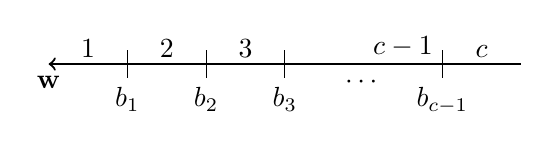
\begin{tikzpicture}
	%\draw[step=1cm,gray,very thin] (-1.9,-1.9) grid (5.9,5.9);
	\draw[thick,<-] (0,0) -- (6,0);
	\foreach \x in {1,2,3}
		\draw (\x cm,5pt) -- (\x cm,-5pt) node[anchor=north] {$b_\x$};
	\node[anchor=north] at (4cm, -1pt) {$\cdots$};
	\draw (5 cm,5pt) -- (5 cm,-5pt) node[anchor=north] {$b_{c-1}$};	
	\node[anchor=north] at (0cm, -1pt) {$\wv$};
	\node[anchor=south] at (0.5 cm, -1pt) {$1$};
	\node[anchor=south] at (1.5 cm, -1pt) {$2$};
	\node[anchor=south] at (2.5 cm, -1pt) {$3$};
	\node[anchor=south] at (4.5 cm, -1pt) {$c-1$};
	\node[anchor=south] at (5.5 cm, -1pt) {$c$};
	\end{tikzpicture}
\end{center}
	
The ordering in the labels is now respected, if we constrain $b_1 \leq b_2 \leq \cdots \leq b_{c-1}$: 
\begin{align}
	\hat y \leq k \implies \hat y \leq l, ~~ \forall~ l \geq k.
\end{align}

We learn the weights $\wv$ and $b_1, \ldots, b_{c-1}$ by reducing to a sequence of (coupled) binary classifications: 
\begin{align}
\label{eq:svor-c}
\min_{\wv, b_1 \leq b_2\leq \cdots \leq b_{c-1}}~ \tfrac{\lambda}{2}\|\wv\|_2^2 + \sum_{k=1}^{c-1} \sum_{i=1}^n \max\{0, 1- (\pred{y_i = k}- \pred{y_i=k+1}) (\inner{\xv_i}{\wv} + b_{k}) \}, 
\end{align}
where recall that $\pred{A}$ is 1 if $A$ is true and 0 otherwise. It is clear that when $c=2$, the above reduces to the familiar soft-margin SVM. \uline{Derive the Lagrangian dual of \eqref{eq:svor-c}}. [If it helps, you may ignore the constraint $b_1 \leq \ldots \leq b_{c-1}$.]

\ans{\vskip8cm
}	


\item (2 pts) In the previous formulation, to learn $b_k$, essentially we take class $k$ as positive and class $k+1$ as negative. Can you find a ``better'' alternative? \uline{Write down the formulation}. [Hint: it would be similar to \eqref{eq:svor-c}.]

\ans{\vskip4cm
}
\end{enumerate}
\end{exercise}

\end{document}
              